\chapter{Implementation}
As the models defined in the previous chapters have not been specified enough, we here 
present the specified surrogate models and methodologies for the upcoming results. Furthermore, 
we shortly explain the implementation details of the Bayesian optimization routine. 

\section{Bayesian Optimization (BO)}\label{BO_implementation}
The Bayesian optimization framework is implemented as a python class. It is possible to pass the class two
different types of problem objects (COCO and sklearn test problems), and additionally, the class
needs to be given one of the defined surrogate models (also an object). By defining the BO methodology
in this modular fashion, we make sure that we are treating all experiments equally. 

The Bayesian optimization procedure used in the experiments is as follows. Initially, 5 data points
are sampled randomly from the domain $\mathcal{X}$ and evaluated in $f(\cdot)$ (all defined in the
problem class). Next, an optimization step is performed repeatedly, until a predefined budget (how
many samples from $f$ the user allows) is used up. The optimization step is simply a fitting
procedure, followed by finding the point $x_{\text{next}}$ which maximizes the acquisition function,
and including the point and the evaluation $f(x_{\text{next}})$ into the dataset. The maximization
of the acquisition function is done by testing $d\cdot 5000$ random points on the domain, where $d$
is the dimension of the problem. The acquisition function used for the experiments is the expected
improvement in closed form, i.e. all surrogate models are approximated by a Gaussian. 

\begin{note2}[Budget]
  In real-life Bayesian optimization, the budget could be time, money, etc. In this thesis we assume
that these utilities are a linear function of the number of function evaluations. Therefore, we
define the budget (used in the upcoming experiments) as the number of function evaluations.
\end{note2}

\section{Surrogates}
All surrogate models are defined as Python classes, with similar function names, i.e.
\textit{predict}, \textit{fit} and \textit{name}, such that they fit into the BO framework
(described in the above section). In the following, we present how all the surrogate models are
implemented. First, we describe the implementation of the discriminative surrogate models (GP, BNN, BOHamiANN). Next,  
we describe the implementation of the generative/mixture surrogate models (GMR, KDE, SPN). 

\subsection{Discriminative surrogates}
The \textbf{Gaussian process (GP)} regression is implemented using the GPy framework, with the Matern kernel with
$\nu=1.5$. The hyperparamteres, i.e. the lengthscale, variance and observation variance are
optimized by maximizing the marginalized likelihood using the limited memory quasi-newton solver
with bounds ($10^{-3}, 2$). l-bfgs-b max 1000 iterations with 20 restarts. 
The bounds are reasonable since the data is always standardized. 

%\subsubsection{BNN}
The \textbf{Bayesian neural network (BNN)} is a fully connected neural network with 3 layers for 50 tanh
nodes. It is implemented using Numpyro - which is a python library for probabilistic machine
learning, developed by some of the people behind Pyro. Different from Pyro, Numpyro uses Jax (and
not PyTorch) as the backend. This allows for a significantly large speedup when doing MCMC, i.e.
NUTS sampling. The MCMC routine is still quite slow and we limit the sampling size to 500 burn-in
samples and 500 (hopefully) posterior samples with 4 chains - this showed good empirical results on
1D problems. The prior distribution for weights and bias is a standard normal distribution. This is
reasonable since the data is always standardized. As we are (mostly) dealing with noise-free problems, 
we put an informative prior of $InvGa(1000,1)$ on the observation variance i.e. giving a very small observation
variance. 

%\subsubsection{BOHamiANN}
The \textbf{BOHamiANN} model is presented in the paper \cite{BOHAMIANN} and is implemented as it is implemented default
in "github.com/automl/pybnn", which is a fully connected Bayesian neural network with 50 tanh nodes on 3 layers. 
I.e. Same architecture as we use for our implementation, BNN. 

\begin{table}[H]
  \centering
  \resizebox{\textwidth}{!}{\begin{tabular}[t]{p{.20\textwidth} | p{.40\textwidth}  | p{.40\textwidth}}
  \textbf{Model}       & \textbf{Specification}    &   \textbf{Training} \\ \hline
  BNN& 
  \begin{tabular}[t]{l}
    3 layers of 50 tanh nodes\\ 
    $p(\textbf{w}, b) \sim \mathcal{N}(0,1)$ \\
    $p(\sigma) \sim \text{InvGa}(1000,1)$ 
  \end{tabular} &
  \begin{tabular}[t]{l}
    NUTS(500 burn-in, 500 samples) 
  \end{tabular} \\\hline

  BOHamiANN& 
  \begin{tabular}[t]{l}
    3 layers of 50 tanh nodes\\ 
    $p(\textbf{w}, b) \sim \mathcal{N}(0, \sigma_{w})$ \\
    $p(\sigma) \sim \text{LogNormal}(??)$ \\
    $p(\sigma_{w}) \sim \text{Gamma}(??)$
  \end{tabular} &
  \begin{tabular}[t]{l}
    Adaptive stochatic HMC \\
    (1000 burn-in, use every 10 of 2000 samples) 
  \end{tabular} \\\hline

  GP& 
  \begin{tabular}[t]{l}
    Mantern kernel 52
  \end{tabular} &
  \begin{tabular}[t]{l}
    Maximize marginalized likelihood \\
    20 restarts of BFGS optimization
  \end{tabular} \\\hline
  \end{tabular}}
  \caption{Overview of chosen discriminative surrogate models 
          }
\end{table}

\subsubsection{Generative surrogates}
We now present how the generative/mixture models (GMR, KDE, SPN) are implemented more concretely. Firstly, 
all the models have some hyperparameters, which we will not fix,  
\begin{itemize}[noitemsep]
  \item GMR: Number of components, prior weight. 
  \item KDE: Variance of x and y components for all component,  prior weight. 
  \item SPN: Prior on the variance of x and y components,  prior weight.
\end{itemize}
We select the hyperparameters using 30 fold (or leave one out for data size smaller) cross-validation, 
where the models are scored on their mean predictive log probability, i.e. uncertainty quantification. 
We test 40 different points using Bayesian optimization outside the crossvalidation loop. This is
done using the Python package "scikit-optimize". 

The prior variance should be sufficiently large, such that the benefit of the model actually fitting the 
the data is larger than just setting the prior weight high. We set the prior variance to 100 (Which is large since the 
data is standardized). 

%\subsubsection{GMR}
The Gaussian mixture regression (GMR) is implemented using the software\cite{GMR}, which takes in
mixture components and weights trained using sklearn's Gaussian mixture model. Which we train using
20 restarts.

%\subsubsection{KDE}
The kernel decision estimator regression is implemented using numpy and fast vector operations. As
mentioned the standard deviation of all is mixture components in the x and y direction is found
using cross-validation in the range between $(10^{-3}, 0.3)$. 

SPN is implemented using software similar to RAT-SPN but implemented by Mikkel N. Schmidt. It is
trained using the EM algorithm to maximize the posterior i.e. finding the MAP estimate. The
posterior is found in closed form since the component distributions are Gaussian and the prior is
given as an inverse gamma (i.e. a conjugate prior). Inverse gamma distributions have two parameter
the shape $\alpha>0$ and the scale $\beta>0$, and a mean, $\frac{\beta}{\alpha-1}$ for $\alpha >1$, 
and a variance $\frac{\beta^2}{(\alpha-1)^2(\alpha-2)}$ for $\alpha >2$. Looking at plots of the
distribution we choose to fix $\beta =1$ and select $\alpha \in [1,200]$ using cross-validation. 

\begin{table}[H]
  \centering
  \resizebox{\textwidth}{!}{\begin{tabular}[t]{p{.20\textwidth} | p{.40\textwidth}  | p{.40\textwidth}}
  \textbf{Model}       & \textbf{Specification}    &   \textbf{Training} \\ \hline
  GMR& 
  \begin{tabular}[t]{l}
    Training sklearn GMM, \\
    EM of MLE with 3 restarts.\\
    pluggin into GMR software \cite{GMR}. 
  \end{tabular} &
  \begin{tabular}[t]{l}
    BO Cross-validation 30 fold, \\
    tuning number of components \\ 
    and prior weight
  \end{tabular} \\\hline

  KDE& 
  \begin{tabular}[t]{l}
    Gaussian around all datapoints \\
    with a x-variance and y-variance
  \end{tabular} &
  \begin{tabular}[t]{l}
    BO Cross-validation 30 fold,\\
     testing x-variance and y-variance and prior weight\\ 
  \end{tabular} \\\hline

  SPN& 
  \begin{tabular}[t]{l}
    Trained using 3 restarts of EM of MAP,\\  
  \end{tabular} &
  \begin{tabular}[t]{l}
    BO Cross-validation 30 fold,\\
     tuning: hyperpriors and prior weight
  \end{tabular} \\\hline

  \end{tabular}}
  \caption{Overview of chosen generative surrogate models  
          }
\end{table}
%\subsection{Model definintions}
Whereas a true Bayesian would not choose a specific type of model, but use all models
, however, this would indeed be infeasible. We need to limit the scope, 
For the GP, we do 20 restarts in the emperical maximization. And the manteen kernel prior
with $\nu = 2.5$. 
BNN, is a 50x50x50 tanh layers with standard Gaussain priors on. And an inverse gamma (1000, 1)
prior on the noise. Trained with 100 burn-in and 100 samples. 
BOHAMIANN is similar but uses a different noise prior, and trains using the adaptive HMC method. 
The mixture models are trained using crossvalidation scored on the mean predictive log .. posterior
(formally speaking this is not a likelihood, but we will keep it as it is almost the same)
The tuning parameters 
We do 40 iterations 
SPN is trained using EM with maximum 1000 epochs (is terminated if the progress is stalling). 
it is trained 2 times. \todo{Lav den historie}
GMR is trained using EM but this is done by the sklearn software. 

\section{Standardized data}
Before the data reach any of the models, it is standardized. this is a scaling and a translation
of the data, such that the datas empirical mean and standard deviation are 0 and 1,
respectively. Using standardized data makes it much easier to control the parameters in the models
since the data used in fitting and prediction is always on the same scale. The first time the models
see the data, the empirical mean and standard deviation are recorded both for $x$ and $y$, (note $x$
can be a vector), giving $\mu_x$,$\mu_y$, $\sigma_x$and $\sigma_y$. When fitting the data, all data
is transformed using the transformation, 

$$T(x,y) := \left(\frac{x-\mu_x}{\sigma_x}, \frac{y-\mu_y}{\sigma_y} \right).$$

When doing prediction i.e. calculating $p(y|x)$, we use the above transform on the input $x$, and
the model output $y$ is transformed back to the original domain using the inverse transform, 
$$T^{-1}_y(\hat y) :=\hat y \cdot \sigma_y+\mu_y.$$

 \chapter{Experimental results}
 In the following chapter, we want to test the surrogate models both as regression models and as surrogate
 models in a Bayesian optimization setting. Firstly, we stay in the 1D domain on self-defined test problems, 
 which will give an intuition about the capability of the generative and discriminative models. 
We have designed 4 test functions, which are defined to give an advantage to all the regression models. Secondly, 
we go to the higher dimensional problems from the BBOB noiseless problem set. This is a popular set of problems 
with 24 different problems for continuous black-box optimization algorithms.


% Bayesian optimization experiments we want to test the performance of as probabilistic regression
% models.
%  Thereby we might find regression models, which is better?! When this is established we want
%  to test out the performance as a Bayesian optimization routine!
 
%  Firstly an overview of the implementation!. 
 
%  \todo{Lav systematiske resultater. Udvælg functionsklasser at kigge på}
 
%  <reproducer resultater fra Arayns thesis>
%  Egne forsøg med SPN og mixture regression

 \section{Regression analysis methodology}
 As described in the previous sections, an essential part of Bayesian optimization and the decision
 theory built around Bayesian optimization is that the regression model is well-fitted. We will therefore
 look at how good the regression models are in terms of accurate prediction and 
 correct uncertainty estimation. The following provides details on how exactly this is done. 

 \subsection{Uncertainty quantification}
Well-calibrated uncertainty estimation is important for a probabilistic regression model. A good fit is
scored on the model's ability to assign a non-zero (hopefully large) probability to every test point, i.e.
we hope for a given test point $(x_t, y_t)$, that $p(y_t|x_t,\mathcal{D})$ is large. 

One way to score the fit on a large test set $(x_t, y_t)_{t=1}^T$, is to simply calculate the average
density assigned to all $y_1, ..., y_T$, i.e. 
$$\text{Score}_1  = \frac{1}{T}\sum_{t=1}^T p(y_t|x_t,\mathcal{D}),$$ 
however, if the regression model is really certain about one test point and guess this point correct,  
we could have potentially $\text{Score}_1 = \infty$ as $ p(y_t|x_t,\mathcal{D})$ could be arbitraty certain about this 
1 point. Meanwhile, test points with no assigned density, i.e $p(y_t|x_t,\mathcal{D}) = 0$, will not matter. 

Another way to score the fit on the large test, is to score the joint predictive density (with assumed iid 
test data), 
$$p(\textbf{y}_T|\textbf{x}_T, \mathcal{D}) = \prod_{y=1}^T p(y_t|x_t, \mathcal{D})$$
Now, if just one test point is assigned zero probability the regression model has failed overall. 
Additional, on a computer with finite-precision small probabilities might underflow to 0 and course
the score to be 0. We overcome underflow with a log transformation and take the mean value to 
compare with different amounts of test data,
$$ \text{Score}_2 = \frac{1}{T} \log p(\textbf{y}_T|\textbf{x}_T, \mathcal{D}) = \frac{1}{T}\sum_{t=1}^T \log p(y_t|x_t, \mathcal{D}).$$
We call this score the \textit{mean log predictive density} and it will be use in the experiments conducted in this thesis. 

\subsection{Predictive power}
The performance of a deterministic regression model $f_w(\cdot)$ is typically measured in mean squared error or 
mean absolute error (MAE), i.e. 
$$MAE = \frac{1}{T}\sum_{t=1}^T |f_{w}(x_t) - y_t|.$$ For the probabilistic regression model, we
want a similar measurement - especially if the uncertainty quantification fails. It makes sense to use
the most probable outcome of the predictive distribution, i.e. the mode. However, if it is Gaussian
the mode is equal the mean. The mean absolut error used in this project is given as, 
$MAE :=\frac{1}{T}\sum_{t=1}^T |\mu_{\mathcal{D}}(x_t) - y_t|.$ However, to make the performance
relateable across problems, we use the mean relative error, 
$$\text{Mean relative error} :=\frac{1}{T}\sum_{t=1}^T \frac{|\mu_{\mathcal{D}}(x_t) - y_t|}{|y_t|}.$$

\subsection{Benchmark surrogate model}
Before moving on with the results, we want to introduce an important benchmark surrogate model, the
\textit{emperical mean and std} model (always plotted in black). This surrogate's predictive distribution
is a simple normal distribution with mean and variance of the training $y$-data i.e. $\textbf{y}$. More
formally it is defined as, 
$$p(y|x\mathcal{D}) = \mathcal{N}(y| \bar{\textbf{y}} , \bar{\sigma}^2 (\textbf{y})),$$ where
$\bar{\textbf{y}} = \frac{1}{n}\sum_{i=1}^n \textbf{y}_i $ and $\bar{\sigma}^2 (\textbf{y}) =
\frac{1}{n}\sum_{i=1}^n (\textbf{y}_i-\bar{\textbf{y}})^2$. In the context of Bayesian optimization,
it is imidiately a bad model since it sees as all $x$ points/locations as equally good. We will use
this model in the benchmark for the Bayesian optimization as it will corespond to random search. 
 
\section{Model comparison on test problems (regression)}
% Experiment section. For each experiment
%  1. Introduction. What is the purpose of the experiment
%  2. Data, materials, methods. Exactly how was the experiment conducted.
%  3. Results
%  4. Discussion. Conclusions.
Bayesian optimization is typically performed on black-box functions, and thereby the Bayesian
regression model is trained on data from all kinds of underlying problems. Now we want to test the
performance of different regression models on different types of 1D problems, all in the interval $x
\in [-100,100]$:

\begin{itemize}
  \item Test 1: A well-behaved sine-function,
  \item Test 2: A highly discontinuous function,
  \item Test 3: A multi-modal objective function,
  \item Test 4: An anisotropic objective function.
\end{itemize}
The functions are illustrated here,

\begin{figure}[h]
  \centering
  \begin{minipage}[b]{0.24\textwidth}
   \includegraphics[width=\textwidth]{Figures/reg_illustrations/all_reg_figures/Test1.pdf}
  \end{minipage}
  \hfill
  \begin{minipage}[b]{0.24\textwidth}
    \includegraphics[width=\textwidth]{Figures/reg_illustrations/all_reg_figures/Test2.pdf}
   \end{minipage}
   \hfill
   \begin{minipage}[b]{0.24\textwidth}
    \includegraphics[width=\textwidth]{Figures/reg_illustrations/all_reg_figures/Test3b.pdf}
   \end{minipage}
   \hfill
   \begin{minipage}[b]{0.24\textwidth}
     \includegraphics[width=\textwidth]{Figures/reg_illustrations/all_reg_figures/Test4b.pdf}
    \end{minipage}

  \label{TEST_problems}
\end{figure}

It is common to have several parameters to tune in Bayesian optimization, but we will first keep the
domain in 1D to establish a more informative evaluation of the model performance. Along with tests of predictive power and
uncertainty quantification, we have figures of the corresponding predictive distribution for every problem, 
model, number of training data and across all 10 random seeds. 

In the following regression tests, we increase the number of training points, i.e. $n_{test} \in$
\{10, 15, 23, 36, 56, 86, 133, 205, 316\}. First, we fit all regression/surrogate models to the
training data. Second, 10000 test points in the $x$-interval $x \in [-100,
100]$ are used to evaluate predictive power (mean relative error) and uncertainty quantification
(mean predictive log density)\footnote{More concretely, we exp-transform this number to make it
easy to plot} for all the models. This is repeated for ten different random seeds to avoid one model
being especially lucky with one instance of the training data. 

%It is 90 regression experiments, since the regression models are tested on
%9 different amont of data point and for 10 different random seeds.

\subsection*{Test1: Well-behaved problem}
The first problem will establish a benchmark since this is a simple function to fit. Its exact definition is,
$$f(x) = x\cdot \sin(\frac{x}{50} \pi) + 150 + \frac{x}{10} + \sin(x) \hspace{0.5cm} x \in [-100,100],$$
giving a smooth wave function, with the optimium around $-77$.

\begin{figure}[bt!]
  \centering
  \begin{minipage}[b]{0.49\textwidth}
   \includegraphics[width=\textwidth]{Figures/results_regression/Test1_dim_1_0.pdf}
  \end{minipage}
  \hfill
  \begin{minipage}[b]{0.49\textwidth}
    \includegraphics[width=\textwidth]{Figures/results_regression/Test1_dim_1_1.pdf}
   \end{minipage}
  \caption{Two different performance measures of all surrogate models as a function of number of
  training data points with 10000 testpoints. Left: Predictive power, i.e. mean relative error
  between predictive mean and the test points (small is better). Right: Uncertainty quantification, measured
  with exponential mean predictive log density (large is better). All lines reprecent the average
  across 10 random seeds.}
  \label{Test1_reg_plot}
\end{figure}

First of all, in Figure \ref{Test1_reg_plot} left, all the methods are performing better than the
mean prediction (black). The average relative error for the mean prediction is constant at 30\%. All
models, besides the Gaussian mixture regression (GMR), have an average relative error of less than
10\% after just 20 training points. Including more data, the Bayesian neural network and the
Gaussian process has the best mean prediction. The third discriminative model, BOHamiANN, seems to
be a "weak learner": After 30 data points, it stays at the same error - even when being presented
for 316 training data points in the end. 

In right plot in Figure \ref{Test1_reg_plot}, the generative models have an increasingly better
uncertainty quantification compared with using the empirical standard deviation (black) after just
20 training points.
%We have been choosing the hyper parameters of the generative models using crossvalidation.
The discriminative models on the other hand perform worse than the empirical standard deviation,
especially the GP is doing exceptionally bad - its overconfident, the reason can be seen in Figure
\ref{Test1_reg_visual_1}, showing one of the 10 regression results from fitting 36 data points. The
GP is so certain on some predictions that it assigns almost 0 preditive density to some of the 10000
test points (i.e the we test all of the line from -100 to 100), yielding very low mean log
predictive density. 
%  The Bayesian neural networks learning curve stagnates around 100 data points, however,
% it provides a decent mean log predictive likelihood. BOHamiANN performs well in the beginning 
% but seems not expressive enough for this task. The architecture of the neural network is besides
% they use a log-normal prior on the variance and a hyper prior on the variance parameter of the weights.
% But it seems like the algorithm does not converge?. The mixture models are crossvalidated to maximize
% the predive likelihood, 
% To get a deeper understanding of Figure \ref{Test1_reg_plot}, we plot one of the 10 runs for 23 data points, 
% in Figure \ref{Test1_reg_visual_1}, and for 56 data points in Figure \ref{Test1_reg_visual_2}.
\begin{figure}[bt!]
  \centering
  \begin{minipage}[b]{0.32\textwidth}
    \begin{overpic}[trim=1cm 0.7cm 1.5cm 0.5cm,clip,width=\textwidth]{Figures/results_regression/Test1/1.pdf}
      \put (10,65) {BNN}
      \put (-5,40) {\small y}
  \end{overpic}
  \end{minipage}
  \hfill
  \begin{minipage}[b]{0.32\textwidth}
    \begin{overpic}[trim=1cm 0.7cm 1.5cm 0.5cm,clip,width=\textwidth]{Figures/results_regression/Test1/2.pdf}
      \put (10,65) {BOHamiANN}
    \end{overpic}
   \end{minipage}
   \hfill
   \begin{minipage}[b]{0.32\textwidth}
    \begin{overpic}[trim=1cm 0.7cm 1.5cm 0.5cm,clip,width=\textwidth]{Figures/results_regression/Test1/4.pdf}
      \put (10,65) {GP}
    \end{overpic}
    \end{minipage}
     
   \begin{minipage}[b]{0.32\textwidth}
    \begin{overpic}[trim=1cm 0.7cm 1.5cm 0.5cm,clip,width=\textwidth]{Figures/results_regression/Test1/3.pdf}
      \put (10,65) {GMR}
      \put (-5,40) {\small y}
      \put (51,5) {\small x}
    \end{overpic}
    \end{minipage}
  \hfill
    \begin{minipage}[b]{0.32\textwidth}
     \begin{overpic}[trim=1cm 0.7cm 1.5cm 0.5cm,clip,width=\textwidth]{Figures/results_regression/Test1/6.pdf}
      \put (10,65) {SPN}
     \end{overpic}
    \end{minipage}
    \hfill
    \begin{minipage}[b]{0.32\textwidth}
      \begin{overpic}[trim=1cm 0.7cm 1.5cm 0.5cm,clip,width=\textwidth]{Figures/results_regression/Test1/5.pdf}
        \put (10,65) {KDE}
      \end{overpic}
      \end{minipage}
  \caption{Plots visualizing all surrogate-models fit of 36 data points (black dots) from Test1
  (black line). This is one of the 90 regression experiments that conduct the results in Figure
  \ref{Test1_reg_plot}. The blue lines encapsulates
  the 95\% credible region. The red line is the predictive mean. The green $\alpha(x) \in [0,1]$
  denote the prior weighting for the generative models.}
  \label{Test1_reg_visual_1}
\end{figure}

\subsection*{Test2: Discontinuous problem}
As GP and BNN have a natural assumption of continuity we want to investigate their performance
on a discontinuous problem. We want to investigate their performance on the folloing step function, 
defined as 
$$f(x) = \sum_{i=1}^{13} u_i \bm{1}(I_{i}\leq x< I_{i+1}) + sin(x) \hspace{0.5cm} x \in ]-100,100]$$
where $\bm{1}$ denoted the indicator function and
\begin{align*}
  I &= \{-100,  -83,  -71,  -60,  -49,  -31,   -9,    3,   14,26,   37,   60,   83,  100\},\\
  u &= \{181, 162, 144,  69, 106,  88, 200, 125, 144, 162, 181,88, 181, 200\}.
\end{align*}
Outside and on the boundaries $\{-100,100\}$ the function value is constant 200. This leads
to a more deficult problem than case 1. 
\begin{figure}[bt!]
  \centering
  \begin{minipage}[b]{0.49\textwidth}
   \includegraphics[width=\textwidth]{Figures/results_regression/Test2_dim_1_0.pdf}
  \end{minipage}
  \hfill
  \begin{minipage}[b]{0.49\textwidth}
    \includegraphics[width=\textwidth]{Figures/results_regression/Test2_dim_1_1.pdf}
   \end{minipage}
  \caption{Left: Predictive power (small is better). Right: Uncertainty quantification (large is
  better). Average across 10 random seeds. More details in Figure \ref{Test1_reg_plot}.}
  \label{Test2_reg_plot}
\end{figure}


In Figure \ref{Test2_reg_plot} left we see that this is indeed harder to fit than Test 1, as
the reative error is not going down as fast. Comparing to Test 1 we here see that the mixtures are
doing as well and sometimes better than the discriminative models. If instead we used the mode for
the mixture regression models, we might see superior performance, as the prediction, will not be
continuous. Looking at the Figure \ref{Test2_reg_plot} right we see the same story as Test1 that the
mixtures regression has the best uncertainty quantification. KDE and SPN (before 100 data points) perfroms better than
Gaussian mixture regression since the mixture components dimensions ($x$ and $y$) does not correlate,
which fits into the data distribution. Same story for BOHamiANN as Test1. 
%The uncertainty quantification 
%of the discriminative takes a jump in the 

\begin{figure}[bt!]
  \centering
  \begin{minipage}[b]{0.32\textwidth}
    \begin{overpic}[trim=1cm 0.7cm 1.5cm 0.5cm,clip,width=\textwidth]{Figures/results_regression/Test2/1.pdf}
      \put (10,65) {BNN}
      \put (-5,40) {\small y}
  \end{overpic}
  \end{minipage}
  \hfill
  \begin{minipage}[b]{0.32\textwidth}
    \begin{overpic}[trim=1cm 0.7cm 1.5cm 0.5cm,clip,width=\textwidth]{Figures/results_regression/Test2/2.pdf}
      \put (10,65) {BOHamiANN}
    \end{overpic}
   \end{minipage}
   \hfill
   \begin{minipage}[b]{0.32\textwidth}
    \begin{overpic}[trim=1cm 0.7cm 1.5cm 0.5cm,clip,width=\textwidth]{Figures/results_regression/Test2/4.pdf}
      \put (10,65) {GP}
    \end{overpic}
    \end{minipage}
     
   \begin{minipage}[b]{0.32\textwidth}
    \begin{overpic}[trim=1cm 0.7cm 1.5cm 0.5cm,clip,width=\textwidth]{Figures/results_regression/Test2/3.pdf}
      \put (10,65) {GMR}
      \put (-5,40) {\small y}
      \put (51,5) {\small x}
    \end{overpic}
    \end{minipage}
  \hfill
    \begin{minipage}[b]{0.32\textwidth}
     \begin{overpic}[trim=1cm 0.7cm 1.5cm 0.5cm,clip,width=\textwidth]{Figures/results_regression/Test2/6.pdf}
      \put (10,65) {SPN}
     \end{overpic}
    \end{minipage}
    \hfill
    \begin{minipage}[b]{0.32\textwidth}
      \begin{overpic}[trim=1cm 0.7cm 1.5cm 0.5cm,clip,width=\textwidth]{Figures/results_regression/Test2/5.pdf}
        \put (10,65) {KDE}
      \end{overpic}
      \end{minipage}

  \caption{Plots visualizing all surrogate-models fit of 36 data points (black dots) from Test2
  (black line). This is one of 90 experiments that conduct the results in Figure
  \ref{Test2_reg_plot}. The blue lines define the 95\% credible region. Predictive mean (red).
  $\alpha(x) \in [0,1]$ is prior weighting (green).}
  \label{Test2_reg_visual}
\end{figure}

\subsection*{Test3: multi-modal problem}
The following problem is corresponding to a multimodal problem, which could occure in simulations with
two equally likely outcomes. We construct this problem to give the mixture models, 
an advantage over the discriminative models. It is defined as follows, 
$$f(x) = 50*g(x)+ 100 + 10*\sin(0.5\cdot x) + \epsilon \cdot (30 - g(x) \cdot 90), \hspace*{0.5cm}x \in
[-100,100],$$ 
where $\epsilon \sim \text{Cat}(0.5,0.5)$ and $g(x) = \text{sign}(x)+1$
($g(x)$ is 0 for negative $x$ and 2 for positive $x$).

\begin{figure}[bt!]
  \centering
  \begin{minipage}[b]{0.49\textwidth}
   \includegraphics[width=\textwidth]{Figures/results_regression/Test3b_dim_1_0.pdf}
  \end{minipage}
  \hfill
  \begin{minipage}[b]{0.49\textwidth}
    \includegraphics[width=\textwidth]{Figures/results_regression/Test3b_dim_1_1.pdf}
   \end{minipage}
  \caption{Left: Predictive power (small is better). Right: Uncertainty quantification (large is
  better). Average across 10 random seeds. More details in Figure \ref{Test1_reg_plot}.}
  \label{Test3_reg_plot}
\end{figure}

In Figure \ref{Test3_reg_plot} left, we see that none of the models are doing better than the mean
prediction. This is obvious since the data is symmetric and jumps randomly between two states. The
Bayesian neural networks are trying the fit the models, the GP is just turning itself into a mean
prediction. In the right plot of Figure \ref{Test3_reg_plot} we see just like previous that the data is parallel with the axis making it perfect
the SPN and KDE to fit. 


\begin{figure}[bt!]
  \centering
  \begin{minipage}[b]{0.32\textwidth}
    \begin{overpic}[trim=1cm 0.7cm 1.5cm 0.5cm,clip,width=\textwidth]{Figures/results_regression/Test3/1.pdf}
      \put (10,65) {BNN}
      \put (-5,40) {\small y}
  \end{overpic}
  \end{minipage}
  \hfill
  \begin{minipage}[b]{0.32\textwidth}
    \begin{overpic}[trim=1cm 0.7cm 1.5cm 0.5cm,clip,width=\textwidth]{Figures/results_regression/Test3/2.pdf}
      \put (10,65) {BOHamiANN}
    \end{overpic}
   \end{minipage}
   \hfill
   \begin{minipage}[b]{0.32\textwidth}
    \begin{overpic}[trim=1cm 0.7cm 1.5cm 0.5cm,clip,width=\textwidth]{Figures/results_regression/Test3/4.pdf}
      \put (10,65) {GP}
    \end{overpic}
    \end{minipage}
     
   \begin{minipage}[b]{0.32\textwidth}
    \begin{overpic}[trim=1cm 0.7cm 1.5cm 0.5cm,clip,width=\textwidth]{Figures/results_regression/Test3/3.pdf}
      \put (10,65) {GMR}
      \put (-5,40) {\small y}
      \put (51,5) {\small x}
    \end{overpic}
    \end{minipage}
  \hfill
    \begin{minipage}[b]{0.32\textwidth}
     \begin{overpic}[trim=1cm 0.7cm 1.5cm 0.5cm,clip,width=\textwidth]{Figures/results_regression/Test3/6.pdf}
      \put (10,65) {SPN}
     \end{overpic}
    \end{minipage}
    \hfill
    \begin{minipage}[b]{0.32\textwidth}
      \begin{overpic}[trim=1cm 0.7cm 1.5cm 0.5cm,clip,width=\textwidth]{Figures/results_regression/Test3/5.pdf}
        \put (10,65) {KDE}
      \end{overpic}
      \end{minipage}

  \caption{Plots visualizing all surrogate-models fit of 36 data points (black dots) from Test3
  (black line). This is one of 90 experiments that conduct the results in Figure
  \ref{Test3_reg_plot}. The blue lines define the 95\% credible region. Predictive mean (red).
  $\alpha(x) \in [0,1]$ is prior weighting (green).}
  \label{Test3_reg_visual}
\end{figure}

\subsection{Test4: Anisotropic problem}
Finally, this problem has a low frequency in the beginning but ends out with a very high frequency.
This is designed to be a difficult problem for the GP as this would need a different lengthscale
throughout the space\footnote{This type of problem motivates GPs with anisotropic kernels such as deep
kernel learning\cite{DeepKernelLearning}.}.

\begin{figure}[bt!]
  \centering
  \begin{minipage}[b]{0.49\textwidth}
   \includegraphics[width=\textwidth]{Figures/results_regression/Test4b_dim_1_0.pdf}
  \end{minipage}
  \hfill
  \begin{minipage}[b]{0.49\textwidth}
    \includegraphics[width=\textwidth]{Figures/results_regression/Test4b_dim_1_1.pdf}
   \end{minipage}
  \caption{Left: Predictive power (small is better). Right: Uncertainty quantification (large is
  better). Average across 10 random seeds. More details in Figure \ref{Test1_reg_plot}.}
  \label{Test4_reg_plot}
\end{figure}

In Figure \ref{Test4_reg_plot} we see that the GP has the best prediction, 

In Figure \ref{Test4_reg_visual} we see that the GP does have a hard time fitting the 36 points, however, when more and more data
becomes dense, the GP will lower its lengthscale and fit the data very well. This is seen in appendix \todo{Appendix}. 

\begin{figure}[bt!]
  \centering
  \begin{minipage}[b]{0.32\textwidth}
    \begin{overpic}[trim=1cm 0.7cm 1.5cm 0.5cm,clip,width=\textwidth]{Figures/results_regression/Test4/1.pdf}
      \put (10,65) {BNN}
      \put (-5,40) {\small y}
  \end{overpic}
  \end{minipage}
  \hfill
  \begin{minipage}[b]{0.32\textwidth}
    \begin{overpic}[trim=1cm 0.7cm 1.5cm 0.5cm,clip,width=\textwidth]{Figures/results_regression/Test4/2.pdf}
      \put (10,65) {BOHamiANN}
    \end{overpic}
   \end{minipage}
   \hfill
   \begin{minipage}[b]{0.32\textwidth}
    \begin{overpic}[trim=1cm 0.7cm 1.5cm 0.5cm,clip,width=\textwidth]{Figures/results_regression/Test4/4.pdf}
      \put (10,65) {GP}
    \end{overpic}
    \end{minipage}
     
   \begin{minipage}[b]{0.32\textwidth}
    \begin{overpic}[trim=1cm 0.7cm 1.5cm 0.5cm,clip,width=\textwidth]{Figures/results_regression/Test4/3.pdf}
      \put (10,65) {GMR}
      \put (-5,40) {\small y}
      \put (51,5) {\small x}
    \end{overpic}
    \end{minipage}
  \hfill
    \begin{minipage}[b]{0.32\textwidth}
     \begin{overpic}[trim=1cm 0.7cm 1.5cm 0.5cm,clip,width=\textwidth]{Figures/results_regression/Test4/6.pdf}
      \put (10,65) {SPN}
     \end{overpic}
    \end{minipage}
    \hfill
    \begin{minipage}[b]{0.32\textwidth}
      \begin{overpic}[trim=1cm 0.7cm 1.5cm 0.5cm,clip,width=\textwidth]{Figures/results_regression/Test4/5.pdf}
        \put (10,65) {KDE}
      \end{overpic}
      \end{minipage}

  \caption{Plots visualizing all surrogate-models fit of 36 data points (black dots) from Test4
  (black line). This is one of 90 experiments that conduct the results in Figure
  \ref{Test4_reg_plot}. The blue lines define the 95\% credible region. Predictive mean (red).
  $\alpha(x) \in [0,1]$ is prior weighting (green).}
  \label{Test4_reg_visual}
\end{figure}

\newpage
\section{Model comparison on test problems (Bayesian Optimization)}
Now we are ready to test the models in a Bayesian optimization setting. Test3 contains multiple
equal minima, and Test4 has a close to minima point on the boundary $x=100$, so testing them would
not be informative. We redefine Test3 and Test4 as seen in Figure \ref{TEST_problems2}. They still
have the same overall structure, so the connecting to the regression analysis should be okay. 

\begin{figure}[b]
  \centering
  \begin{minipage}[b]{0.24\textwidth}
   \includegraphics[width=\textwidth]{Figures/reg_illustrations/all_reg_figures/Test1.pdf}
  \end{minipage}
  \hfill
  \begin{minipage}[b]{0.24\textwidth}
    \includegraphics[width=\textwidth]{Figures/reg_illustrations/all_reg_figures/Test2.pdf}
   \end{minipage}
   \hfill
   \begin{minipage}[b]{0.24\textwidth}
    \includegraphics[width=\textwidth]{Figures/reg_illustrations/all_reg_figures/Test3c.pdf}
   \end{minipage}
   \hfill
   \begin{minipage}[b]{0.24\textwidth}
     \includegraphics[width=\textwidth]{Figures/reg_illustrations/all_reg_figures/Test4c.pdf}
    \end{minipage}
  \caption{All test function used in Bayesian Optimization. We redefine Test3 and Test4.}
  \label{TEST_problems2}
\end{figure}

The Bayesian optimization algorithm is given five initial training data points i.e. $\{(x_1, y_1),
\dots, (x_5, y_5)\}$ corresponding to 5 objective function evaluations. Next the first BO
optimization step is done: First, the surrogate model is fitted, the resulting predictive
distribution is approximated by a Gaussian, and then the expecpected improvement (in closed form)
select the next location, finally we sample $y_6$ from $f(x_{\text{next}})$ i.e.
$\text{Observe}(x_{\text{next}})$. This procedure is repeated untill the \textit{budget}, which we
here define as number of objective function evaluations allowed, is exhasuted. 


To avoid 
lucky optimization paths 

Bayesian optimization using 20 restarts, 
 a more sound analysis would be to use introduce statistics around the tests. however, this also becomes messy quickly. 



% we see that the GP is in fact the best model in the simple
% problem Test1; however, for the more complicated problems, the GP is not the preferred model. 

\begin{figure}[H]
  \centering
  \begin{minipage}[b]{0.49\textwidth}
   \includegraphics[width=\textwidth]{Figures/results_baysopt/Test1.pdf}
  \end{minipage}
  \hfill
  \begin{minipage}[b]{0.49\textwidth}
    \includegraphics[width=\textwidth]{Figures/results_baysopt/Test2.pdf}
   \end{minipage}
   \begin{minipage}[b]{0.49\textwidth}
    \includegraphics[width=\textwidth]{Figures/results_baysopt/Test3c.pdf}
   \end{minipage}
   \hfill
   \begin{minipage}[b]{0.49\textwidth}
     \includegraphics[width=\textwidth]{Figures/results_baysopt/Test4c.pdf}
    \end{minipage}
  \caption{Bayesian optimization of the Test functions average accross 20 different samples of initial dataset of size 5.}
  \label{Test_bayesOpt}
\end{figure}
% Recall that assigning 0 variance to a prediction problem in expected improvement only yeilds a value in the
% expected improvement if it is increasing. 
In Figure \ref{Test_bayesOpt} it is important first of all compare the surrogates to the black random search, e.g.
all of the models did worse than random search in Test3 (bottom left plot in \ref{Test_bayesOpt}).

Comparing the BO of Test3 with the regression analysis at Figure \ref{Test3_reg_plot}, all the
regression models had the same (insufficient) predictive power as the empirical mean benchmark
model. In Bayesian optimization, the regression model is important for exploitation, however, if it
has no predictive power, then the BO on Test3(bottom left plot in \ref{Test_bayesOpt}) shows that
random search is better, as it does not bias toward any parts of the space. Noticeably, the GP in
Test3 is the worst model (together with BOHamiANN) after 16 function evaluations. The generative
models perform almost as good at random search, which is explained by their good uncertainty
quantifications in Figure \ref{Test3_reg_plot} left.

Test1 is the benchmark
and here it becomes evident that BOHamiANN does not work, and GMR is as good as Random search. GP is a clear winner of test1. 

Test 2 shows after 35 iterations that random search is better than the GP and that all the mixture models and (barely) the BNN 
performs better than the GP. 

Finally, test4 shows approximatly the same results for KDE, SPN, BNN and GP, all being better than Random 
search and BOHamiANN. 



, and the uncertainty quantification was good
for the mixture models, and

\section{Test on BBOB in higher dimensions}
So far, we have looked at our self-defined 1D problems and can conclude that our regression models
work and that there exist problems in 1D where the GP is not the preferred model - in fact for Test2,Test3
and Test4. We now want to go up in higher dimensions to test the models on more realistic problems.
The tests are conducted on 2,3,5,10 dimensions on the \textit{Real-parameter black-box optimization
benchmarking 2009: Noiseless functions definitions} (BBOB) \cite{hansen2009real}, which consists for
24 functions divided into 5 different categories of difficulty and are scaleable in dimensions.
These functions are available through Comparing Continuous Optimizers framework COCO \cite{COCO},
which is a popular benchmarking testbed for continuous black-box optimization algorithms. Due to
time and resource constraints on this thesis, we select the functions, f3, f9, f15 and f21 which are
plotted in 2D in Figure \ref{COCO_tests}.
\begin{itemize}[noitemsep]
  \item f3: Rastrigin Function.
  \item f9: Rotated Rosenbrock Function.
  \item f15: Rastrigin Function transformed to be non-separable
  \item f21: Gallagher’s Gaussian 101-me Peaks Function.
\end{itemize}
For more details, all the 24 functions are described here \cite{hansen2009real}. First, we test the
regression performance of surrogate models on the four benchmark problems in dimensions 2,3,5,10.
Secondly, we test Bayesian optimization on them. 

\begin{figure}[h]
  \centering
  \begin{minipage}[b]{0.24\textwidth}
   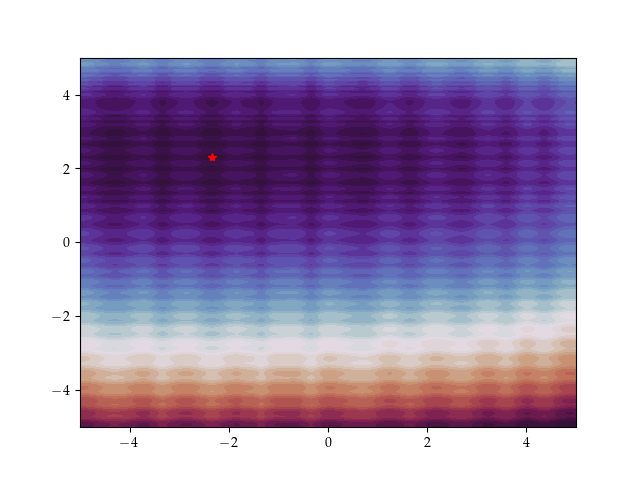
\includegraphics[trim=2.5cm 1.3cm 2.5cm 1.3cm,clip,width=\textwidth]{Figures/coco/f3.png}
  \end{minipage}
  \hfill
  \begin{minipage}[b]{0.24\textwidth}
   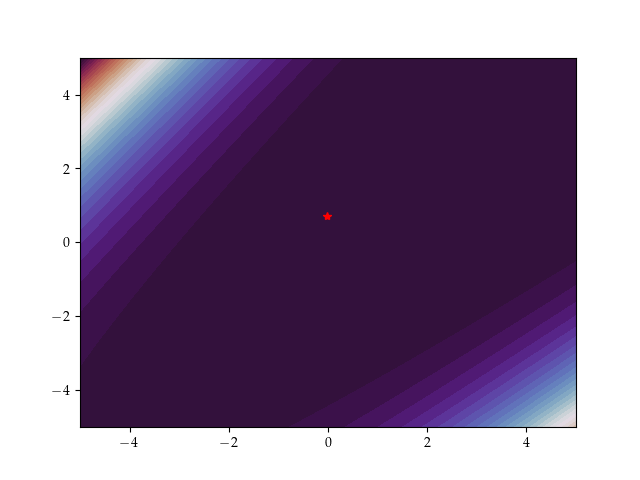
\includegraphics[trim=2.5cm 1.3cm 2.5cm 1.3cm,clip,width=\textwidth]{Figures/coco/f9.png}
  \end{minipage}
  \hfill
  \begin{minipage}[b]{0.24\textwidth}
    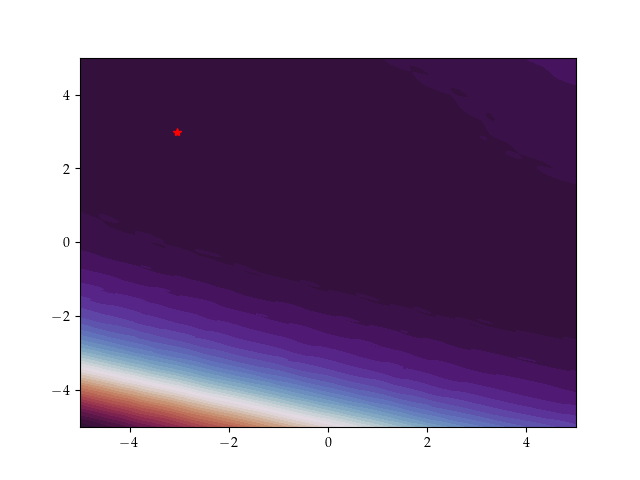
\includegraphics[trim=2.5cm 1.3cm 2.5cm 1.3cm,clip,width=\textwidth]{Figures/coco/f15.png}
    %\caption{Rank}
  \end{minipage}
  \hfill
  \begin{minipage}[b]{0.24\textwidth}
    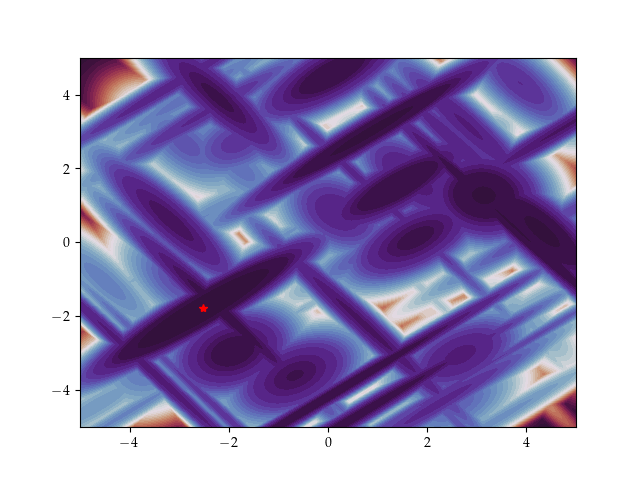
\includegraphics[trim=2.5cm 1.3cm 2.5cm 1.3cm,clip,width=\textwidth]{Figures/coco/f21.png}
  \end{minipage}
  
  \caption{COCO Test functions f3, f9,f15, and f21 in 2 dimensions}
  \label{COCO_tests}
\end{figure}

\subsection{Regression performance on BBOB}
The testing regression performance is the same procedure as the 1D test problems. With 10 seeded random
samples, we select $\{10, 15, 23, 36, 56, 86, 133, 205, 316\}$ points to fit the 4 BBOB problems in 4 dimensions
(2,3,5,10). All results can be seen in the Appendix. The results are in general just like the 1D test problems, 
that the GP has the best predictive power, the uncertainty quantification is, however, more equal between
the generative and discriminative models. We have selected some noticeable plots here. 

\begin{figure}[H]
  \centering
  \begin{minipage}[b]{0.32\textwidth}
   \includegraphics[width=\textwidth]{Figures/results_regression/f3_dim_5_0.pdf}
  \end{minipage}
  \hfill
  \begin{minipage}[b]{0.32\textwidth}
    \includegraphics[width=\textwidth]{Figures/results_regression/f21_dim_3_0.pdf}
   \end{minipage}
   \hfill
   \begin{minipage}[b]{0.32\textwidth}
    \includegraphics[width=\textwidth]{Figures/results_regression/f15_dim_2_0.pdf}
   \end{minipage}
   
     \begin{minipage}[b]{0.32\textwidth}
   \includegraphics[width=\textwidth]{Figures/results_regression/f3_dim_5_1.pdf}
  \end{minipage}
  \hfill
  \begin{minipage}[b]{0.32\textwidth}
    \includegraphics[width=\textwidth]{Figures/results_regression/f21_dim_3_1.pdf}
   \end{minipage}
   \hfill
   \begin{minipage}[b]{0.32\textwidth}
    \includegraphics[width=\textwidth]{Figures/results_regression/f15_dim_2_1.pdf}
   \end{minipage}
   
  \caption{Regression performance of 4 selected out of 12 problems of BBOB (f3,f9,f15,f21 in
  dimensions 2,3,5). All plots are in Appendix \ref{BBOB_regression_all}. Top: Predictive power. Bottom: Uncertainty
  quantification. More details in Figure \ref{Test1_reg_plot}. Average across 10 different samples
  of seeded samples from the problems.}
  \label{BBOB_regression}
\end{figure}


\subsection{Bayesian optimization performance on BBOB}
The Bayesian optimization procedure is as follows: 1) sample 5 random points, 2) do 30 Bayesian
optimization iterations. We want to limit optimization paths of being lucky by doing 20
restarts (preferable more, however, due to time and resource limitations). The optimization of the
acquisition function is done by $d \cdot 5000$ random guesses. To be fairer across the dimensions,
this should have been $5000^d$; however, this would have been computational infeasible. 

\begin{figure}[H]
  \centering
  \begin{minipage}[b]{0.49\textwidth}
   \includegraphics[trim=0cm 2cm 0cm 0.4cm,clip,width=\textwidth]{Figures/results_baysopt/3_2.pdf}
  \end{minipage}
  \hfill
  \begin{minipage}[b]{0.49\textwidth}
    \includegraphics[trim=0cm 2cm 0cm 0.4cm,clip,width=\textwidth]{Figures/results_baysopt/9_2.pdf}
   \end{minipage}
   \begin{minipage}[b]{0.49\textwidth}
    \includegraphics[width=\textwidth]{Figures/results_baysopt/15_2.pdf}
   \end{minipage}
   \hfill
   \begin{minipage}[b]{0.49\textwidth}
     \includegraphics[width=\textwidth]{Figures/results_baysopt/21_2.pdf}
    \end{minipage}
  \caption{Bayesian optimization of BBOB in 2 dimensions, average accross 20 different samples of initial dataset of size 5)}
  \label{BBOB_bayesOpt}
\end{figure}

\begin{figure}[H]
  \centering
  \begin{minipage}[b]{0.49\textwidth}
   \includegraphics[trim=0cm 2cm 0cm 0.4cm,clip,width=\textwidth]{Figures/results_baysopt/3_3.pdf}
  \end{minipage}
  \hfill
  \begin{minipage}[b]{0.49\textwidth}
    \includegraphics[trim=0cm 2cm 0cm 0.4cm,clip,width=\textwidth]{Figures/results_baysopt/9_3.pdf}
   \end{minipage}
   \begin{minipage}[b]{0.49\textwidth}
    \includegraphics[width=\textwidth]{Figures/results_baysopt/15_3.pdf}
   \end{minipage}
   \hfill
   \begin{minipage}[b]{0.49\textwidth}
     \includegraphics[width=\textwidth]{Figures/results_baysopt/21_3.pdf}
    \end{minipage}
  \caption{Bayesian optimization of BBOB in 3 dimensions average accross 20 different samples of initial dataset of size 5)}
  \label{BBOB_bayesOpt}
\end{figure}


\begin{figure}[H]
  \centering
  \begin{minipage}[b]{0.49\textwidth}
   \includegraphics[trim=0cm 2cm 0cm 0.4cm,clip,width=\textwidth]{Figures/results_baysopt/3_5.pdf}
  \end{minipage}
  \hfill
  \begin{minipage}[b]{0.49\textwidth}
    \includegraphics[trim=0cm 2cm 0cm 0.4cm,clip,width=\textwidth]{Figures/results_baysopt/9_5.pdf}
   \end{minipage}
   \begin{minipage}[b]{0.49\textwidth}
    \includegraphics[width=\textwidth]{Figures/results_baysopt/15_5.pdf}
   \end{minipage}
   \hfill
   \begin{minipage}[b]{0.49\textwidth}
     \includegraphics[width=\textwidth]{Figures/results_baysopt/21_5.pdf}
    \end{minipage}
  \caption{Bayesian optimization of BBOB in 5 dimensions average accross 20 different samples of initial dataset of size 5.}
  \label{BBOB_bayesOpt5}
\end{figure}

In large dimensions there are need for more data for the regression model to be correct? Course of dimensionality..?


In general, across the BBOB tests, we see that GP is the best surrogate model. The other models 
are doing worse than random search on several tests. This is unfortunate.